\chapter{Uplift Modelling}
\label{ch-uplift}



This chapter is based 
on 
many references,
including Ref.\cite{uplift-2017, fei, wiki-uplift,jaros}.

\begin{figure}[h!]
$$\begin{array}{ccc}
\xymatrix{
&\rvx\ar[dr]
\\
\rvd\ar[rr]
&&\rvy
}
&\quad&
\xymatrix{
&\rvx\ar[dr]
\\
\rvy_0\ar[rr]
&&\rvy
}
\\
(a) &\quad & (b)
\end{array}
$$
\caption{Bnets for Uplift Modelling (UM). 
Bnet $(a)$ is for a RCT experiment measuring ATE and Bnet $(b)$ is for one measuring Uplift. 
 Since we assume an RCT, the arrows $\rvx\rarrow \rvd$ 
and $\rvx\rarrow \rvy_0$ have been amputated (i.e., removed). This is equivalent to assuming that $P(d|x)=P(d)$ and
$P(y_0|x)=P(y_0)$.
}
\label{fig-up-bnet}
\end{figure}



{\bf Uphill Modelling} (UM) (a.k.a., {\bf Uplift Marketing})
is an experiment that performs an
RCT and other measurements. It 
entails performing an
RCT and 
 calculating  the ATE or Uplift for that  RCT.
 Besides that, UM entails 
separating 
individuals or strata of individuals according to their \qt{UM-type}\footnote{ACE, Uplift and UM-type to be defined later.}



Fig.\ref{fig-up-bnet} shows bnets for 2 experiments. Bnet $(a)$\footnote{
Note that bnet \ref{fig-up-bnet}$(a)$ 
is the bnet for Rubin's theory of 
Potential Outcomes (PO).
PO, which is
discussed in Chapter \ref{ch-pot-out},
 is a subset
of Pearl's Causal Inference.
Besides UM, other  applications of PO theory
that are discussed in this book 
are: Regression Discontinuity (Chapter \ref{ch-reg-dis}),
Difference-in-Differences (Chapter \ref{ch-did})
and Synthetic Controls (Chapter \ref{ch-syn-con}).} is for a RCT experiment measuring ATE and Bnet $(b)$ is for one measuring Uplift. 
The node variables of bnets $(a)$ and $(b)$ of Fig.\ref{fig-up-bnet}
are defined as follows:

$x=(x_0, x_1,\dots, x_{n-1})$ is an $n$ dimensional 
vector of features $x_i$. If any of the $x_i$
is a priori continuous, we will
assume it has  been binned into
a finite number of bins.
Let $val(\rvx)$ be the finite set of  all feature vectors.

$\rvd\in\bool$ equals 1 iff voter receives
a brochure (which
we will call the intervention) trying to convince him/her to vote 
for the target  candidate. The cohort with $\rvd=0$ is called the control group. The one with $\rvd=1$ is called the treated group.
The intervention occurs between times $t_0$ and $t_1$
where $t_0<t_1$.

$\rvy_0=\rvy_{t_0}\in \bool$. Whether a voter would
vote for a candidate at time $t_0$.

$\rvy=\rvy_{t_1}\in \bool$. Whether a voter would
vote for a candidate at time $t_1$. This is also
the treatment response.

Although we are referring to bnets $(a)$
and $(b)$ as 2 different experiments, they can be done
simultaneously. Enacting
bnet $(a)$ requires splitting the initial 
randomized population into two equal parts;
the control cohort and the treated one.
The control cohort is not treated (its members do
not receive the persuasive brochure or treatment). On the other hand, enacting bnet $(b)$ requires
sending all its customers a brochure/treatment,
and sending a questionnaire to all 
customers before and after treatment.
Hence, one can use the treated cohort of
bnet $(a)$ as the full cohort of bnet $(b)$.

For bnet $(a)$, 
\beq
P(y, d, x) = P(y|d,x)P(d)P(x)
\eeq
and for bnet $(b)$,
\beq
P(y, y_0, x) = P(y|y_0,x)P(y_0)P(x)
\eeq

Usually, $P(d) = \frac{1}{2}$.


\section{Uplift experiment}
In this section, we will consider an UM 
uplift experiment of type $(b)$.
in the next section, we will
consider an UM ATE experiment of type $(b)$.

\subsection{Uplift definition}

\begin{figure}[h!]
\centering
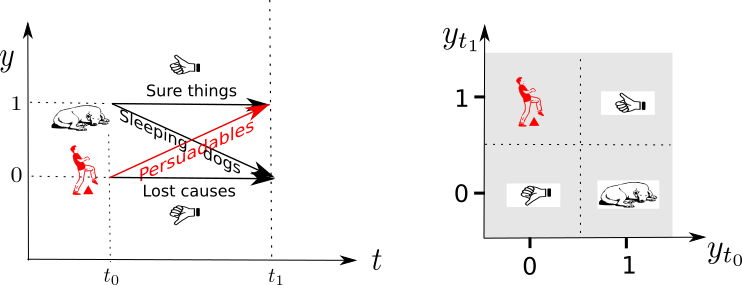
\includegraphics[width=6in]
{uplift/uplift-y-t-up.png}
\caption{UM-intervention
can be used to classify
all customers of the
population into 4 UM-types.
This figure 
assumes $y\in \bool$.
More generally, $y\in \RR$.
$t$ represents time. $t=t_0$
corresponds to $d=0=untreated$,
and $t=t_1$ corresponds to $d=1=treated$.} 
\label{fig-uplift-y-t}
\end{figure}

Let us denote each {\bf customer} (i.e., {\bf participant},  {\bf sample}) 
by $\s$,
where 
\beq\s\in \Sigma=\{0,1,2, \ldots, nsam-1\}
\eeq

Let $y^\s_t\in \RR$ for $t=t_0, t_1$
be whether 
 customer (i.e., sample) $\s$
 will vote for a candidate at time $t$. 
Let $\rvy_{t_1}^\s=\rvy^\s$.
We will call 

\beq
\delta^\s=
y^\s_{t_1}-y^\s_{t_0} = y^\s-y^\s_0
\eeq
the {\bf uplift
for customer $\s$}.
Also, we will call

\beqa
\delta_x &=& \sum_{y, y_0}(y - y_0)P(y, y_0|x)
\\
&=& 
\underbrace{\sum_{y}yP(y|x)}_{\av{\rvy}_x}
- 
\underbrace{\sum_{y_0}y_0P(y_0|x)}_{\av{\rvy_0}_x}
\eeqa
the {\bf uplift for stratum $x$}.
Note that $P(y_0|x)= P(y_0)$ by assumption so

\beq
\av{\rvy_0}_x = \av{\rvy_0}
\eeq
Note also that if $y, y_0\in \bool$,

\beq
\delta_x = P(\rvy=1|x) - P(\rvy_0=1|x)
\eeq

Note also that even when $y, y_0\in\bool$,
their averages  might be a non-integer.

\subsection{UM customer and stratum types}
\label{sec-up-types}
As shown
in Fig.\ref{fig-uplift-y-t},
UM classifies customers
into 4 {\bf UM-types}: Persuadables, SureThings, LostCauses,
and SleepyDogs.
The UM-type
of a customer
depends on the changes 
that are induced on that customer
by an {\bf UM-intervention}.
\begin{itemize}
\item
For a {\bf Persuadable} customer,
$\delta^\s>0$.
\item
For a {\bf SleepyDogs}
customer, $\delta^\s< 0$.
\item
For a {\bf SureThings} customer,
 $\delta^\s\approx 0$
and $y^\s_{t_0}$ is high.
\item
For a {\bf LostCauses} customer,
$\delta^\s\approx 0$
and $y^\s_{t_0}$ is low.
\end{itemize}

Let $A_x = \{\s: x^\s \approx x\}$ for  $x\in val(\rvx)$.
The set $A_x$ of all samples with
a feature vector $x^\s$ close to $x$ 
is called the $x$ {\bf stratum}.

Strata can also be
classified into
the 4 UM-types. To do
so, replace $\delta^\s$ by $\delta_x$
and $y^\s_{t_0}$ by $\av{\rvy_0}$
in the definitions given above for the 4 UM-types.
A customer 
may not be typical for
his stratum
and may
have different
{\bf customer and stratum UM-types}.
For example, he may have positive 
customer uplift $\delta^\s$
and therefore have a Persuadable customer UM-type,
but his stratum-uplift  $\delta_x$
might be negative, so
he has
the SleepyDogs stratum UM-type.

Advertisers are very interested in finding
the Persuadable stratum in a population
so as to focus their resources on them.
For example, UM was used very
successfully during the 
Obama presidential campaigns. 
Team Obama conducted UM-interventions.
This allowed them to
identify voters who might be sitting on the fence
on whether to vote for Obama.
Then Team Obama spent
the lion share
of  resources  on those
fence-sitters.



\subsection{Stratum ranking}
\label{sec-up-ranking}

The input
to an uplift experiment $(b)$ is a PO
dataset $DS= \{ (\s, d^\s, x^\s,  y):
 \s\in\Sigma\}$.
 
\begin{figure}[h!]
\centering
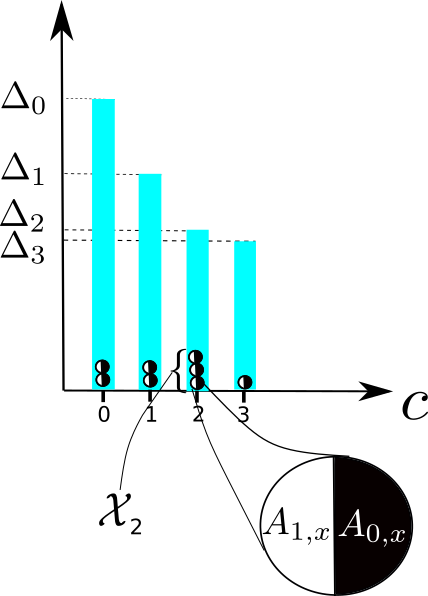
\includegraphics[width=2in]
{uplift/uplift-bins-up.png}
\caption{
Pictorial
representation
of the sequence
$\{(\calx_c, \Delta_c)\}_{c=0, 1, \ldots, nc-1}$.
}
\label{fig-uplift-bins}
\end{figure}


Starting with $DS$,
UM performs the following steps.
Fig.\ref{fig-uplift-bins}
is a pictorial representation
of the quantities
that are calculated
during these steps.

\begin{enumerate}
\item Find 

\beq
A_x = \{\s: x^\s \approx x\}\eeq
for each observed $x\in val(\rvx)$.
Set $A_x=\emptyset$ for unobserved $x\in val(\rvx)$.
 
\item Use Eq.(\ref{eq-est-ace-uplift})
to calculate $\delta_x$
for each $x\in val(\rvx)$.
Set $\delta_x=0$ if $A_x=\emptyset$.

\item Partition 
the set $\{\delta_x: x\in val(\rvx)\}$
into disjoint bins. Call
$\Delta_c$  the average $\delta_x$ 
within bin $c$ for $c=0, 1, \ldots, nc-1$.
The class labels 
$c$ should be assigned
so that the sequence of
$\Delta_c$
is monotonic and non-increasing; i.e.,

\beq
\Delta_0 \geq \Delta_{1}\geq\cdots \geq \Delta_{nc-1}
\;.
\eeq
Now calculate 

\beq
\calx_c =\{ x: \delta_x \approx \Delta_c\}
\eeq
 for each $c$.
By the end of this step,
we will have calculated 
$\{(\calx_c, \Delta_c)\}_{c=0, 1, \ldots, nc-1}$
from $\{(x, \delta_x)\}_{x\in val(\rvx)}$.
We will refer to the $\calx_c$
as {\bf stratum-bins}. Note that
\beqa
\Delta_c &=&\frac{1}{|\calx_c|}\sum_{x\in\calx_c}\delta_x
\\
&=&
\underbrace{\frac{1}{|\calx_c|}\sum_{x\in\calx_c}\av{\rvy}_x}_
{\displaystyle Y^1_c}
- 
\underbrace{\frac{1}{|\calx_c|}\sum_{x\in\calx_c}\av{\rvy_0}_x}_
{\displaystyle Y^0_c}
\;.
\label{eq-Delta-c}
\eeqa
\item
For each $c$,
calculate 

\beq
A_{x,y_0}=\{\s\in A_x: y_0^\s = y_0\}
\eeq

\beq
\Sigma_{y_0,c}=\cup_{x\in \calx_c}A_{x,y_0}
\eeq
for $y_0\in\bool$
and 

\beq
\Sigma_{c}=\Sigma_{0,c}
\cup \Sigma_{1,j}
\;.
\eeq
\end{enumerate}


\begin{figure}[h!]
\centering
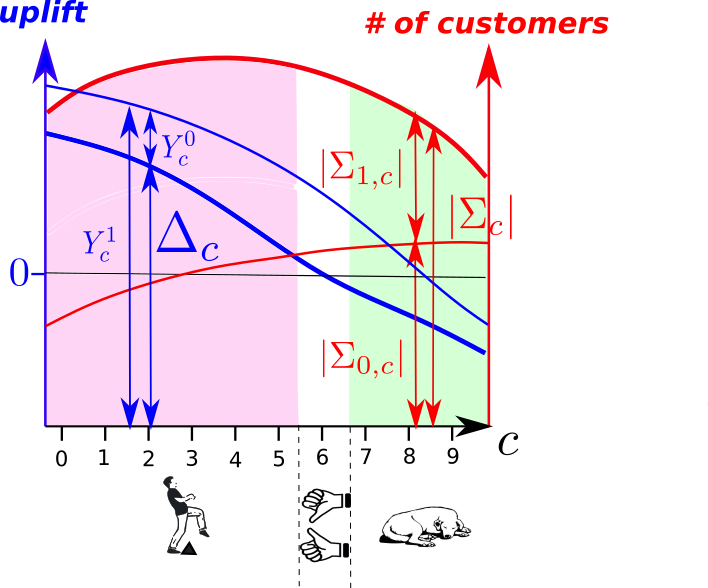
\includegraphics[width=4in]
{uplift/qini-fake-up.png}

\caption{
Plot
of UM results.
} 
\label{fig-qini-fake}
\end{figure}
Fig.\ref{fig-qini-fake}
is a  way of
plotting
the results 
of UM in an
intuitive
way.


Another common plot of UM results is
called a {\bf Qini
curve}.
A Qini curve is a plot 
of $(X_c,Y_c)$
for all $c$, where

\beq
X_c= \sum_{c'=0}^{c}\sum_{x\in \calx_{c'}}|A_x|
\eeq
is the cumulative population (counting the
samples in
order of decreasing uplift) and

\beq
Y_c=\sum_{c'=0}^c \Delta_{c'}
\eeq
is the cumulative uplift.
As $c$ increases, a Qini curve rises fast at first and then its slope decreases until
at some value $c_0$, the slope is defined as too small to care. No marketing resources are
directed towards
customers $\s$ for whom  $c>c_0$.\footnote{
Let 
$S_{\Delta} = \{\s:\delta^\s \geq \Delta\}$.
A Qini curve can also be defined, without stratification,
as a
 plot of $(X_\Delta, Y_\Delta)$ for all $\Delta>0$,
where $
X_\Delta = |S_{\Delta}|$
and
$
Y_\Delta= \sum_{\s\in S_{\Delta}}\delta^\s
$. As $\Delta$ decreases, a Qini curve rises fast at first and then its slope decreases.
}

\section{ATE experiment}
\subsection{ATE definition}

$ATE=$ Average Treatment Efect

$ACE =$ Average Causal Effect

$ATE=ACE$

Recall
the following technical formulae
that were proven in 
Chapter \ref{ch-pot-out}:



\begin{itemize}

\item
Recall Eq.(\ref{eq-ace-propensity}):

\beq
ATE =\sum_x P(x)
\underbrace{
\sum_y y\left[
P(y|d=1, x)
-
P(y|d=0, x) 
\right]
}_{ATE_x}
\eeq
If $\rvy\in \bool$, then

\beq
ATE_x
=
\underbrace{
P_{\rvy|\rvd, \rvx}(1|1, x)
}_{\displaystyle Y^1_x}
-
\underbrace{
P_{\rvy|\rvd, \rvx}(1|0, x)
}_{\displaystyle Y^0_x}
\;.
\eeq

\item
Recall 
Eq.(\ref{eq-ace-esti-posi}):

\beq
\HAT{ATE_x}
=
\underbrace{
\frac{1}{N_x}
\sum_{\s \in A_x}
\frac{d^\s y^\s}{g_{1|x^\s} }
}_
{\displaystyle Y_x^1}
-
\underbrace{
\frac{1}{N_x}
\sum_{\s \in A_x}
\frac{(1-d^\s)y^\s}{g_{0|x^\s} }
}_
{\displaystyle Y_x^0}
\label{eq-est-ace-uplift}
\eeq

\end{itemize}

\subsection{Replacing Uplift by ATE}
In section \ref{sec-up-types} (entitled \qt{\nameref{sec-up-types}})
and section \ref{sec-up-ranking} (entitled 
\qt{\nameref{sec-up-ranking}}),
we can replace Uplift by ATE, if we replace:

\beq
\delta_x\rarrow ATE_x,\quad \av{\rvy}_x\rarrow Y_x^1,\quad
\av{\rvy_0}_x\rarrow Y_x^0, \quad y_0\rarrow d
\eeq
in all the formulae and figures.

This means that we can rank strata by their $ATE_x$ instead of
their $\delta_x$. Note, however, that individual customers
have an individual uplift $\delta^\s$, but they don't have an
individual $ATE^\s$.
Uplift types
can be defined at an individual level
($y^\s$ and
$y^\s_0$ are both available), whereas ATE typing can't
($y^s$ is not available for both $d^\s=0,1$).


